\chapter{Aplikacja demonstracyjna}
\label{chapter:app}

\section{Opis aplikacji wspomagającej warsztat samochodowy}

	Aplikacja przygotowana jako część praktyczna pracy dyplomowej powstała z uwagi na kilka
	czynników. Głównym powodem była chęć dostarczenia aplikacji, której zadaniem jest wsparcia
	dla przedsiębiorstwa prowadzącego warsztat samochody. Ponadto chęć poznania framework'a jakim
	jest \textbf{Spring}, zrozumienia zasad jakimi rządzi pisania się dużej aplikacji zdecydowały
	o wyborze takiego, a nie innego tematu. 
	
	Nadrzędnym celem aplikacji jest wsparcia dla misji przedsiębiorstwa prowadzącego warsztat
	samochody zajmujący się serwisowaniem samochodów, prowadzącym naprawy oraz przegląd oraz
	dokonującym okresowych czynności eksploatacyjnych jak na przykład wymiana oleju czy filtrów.
	Z tego powodu w kolejnych modułach aplikacji została zrealizowana część zarówno serwerowa jak i 
	kliencka, które dostarczają funkcjonalność pozwalających na tworzenie, edycję oraz usuwaniu 
	obiektów biznesowych jak i również przeglądanie informacji o nich.

	Duży nacisk został położony na zrealizowanie warstwy serwerowej z uwagi na jej krytyczne znaczenie.
	Jest ona odpowiedzialna za realizacji postulatów logiki biznesowej, zarządzania prawami dostępu,
	walidację i konwersję danych. Z uwagi na wymienione punkty wiele elementów zostało dopracowanych, a 
	poszczególne autorskie implementacje pewnych problemów zastąpione lepiej przetestowanymi i wydajniejszymi
	bibliotekami lub framework'ami. 
		
	\subsection{Funkcjonalność aplikacji}
	Istniejąca funkcjonalność aplikacji pozwala na:
	\begin{enumerate}
		\item dostęp do niektórych funkcji aplikacji dostępny jest jedynie dla osób upoważnionych:
		\begin{itemize}
			\item aplikacja rozpoznaje czy użytkownik jest zalogowany czy nie dostosowując ilość dostępnych funkcji,
			w zależności od grupy (grup) w których użytkownik się znajduje,
			\item na obecną chwilę weryfikacja następuje jedynie po adresie URI który uruchamia daną akcję
		\end{itemize}
		\item możliwe jest tworzenie nowych spotkań oraz raportów,
		\item możliwe jest przeglądania terminarza spotkań,
		\item istnieje generyczna warstwa stron obiektów domenowych, gdzie jedynym wymogiem jest istnienie obiektu w bazie
		oraz poprawność adresu
	\end{enumerate}
		
	\subsection{Architektura MVC}
		Aplikacja została zrealizowana w architekturze MVC. Architektura MVC jest znanym wzorcem projektowym
		szczególnie użytecznym w procesie projektowania warstwy widoku. Korzyści takie jak odseparowanie logiki biznesowej,
		warstwy modelu danych czy też ostatecznie faktycznej funkcjonalności aplikacji udostępnionej poprzez serwisy. 
		Model danych jest odpowiedzialny za zamknięcie i przenoszenie danych. W rozumieniu omawianego paradygmatu widok służy
		jedynie do zaprezentowania danych Warstwa środkowa - kontrolery jest często utożsamiana jak najważniejsza część z uwagi
		na jej położeniu. Kontrolery odbierają żądania wysyłane przez klientów i wywołania serwisów celem uzyskania danych
		do wygenerowania poprawnej odpowiedzi, aby mogły być zaprezentowane w warstwie widoku\cite{spring_recipies}.
		
		W użytym szkielecie aplikacji - \textbf{Spring MVC}\ref{app:spring_mvc} - model jest zbiorem \textit{domain objects}\footnote{
		\textbf{Domain Object} - obiekt biznesowy będący encją zawierającą informacje użyteczne z punktu widzenia logiki biznesowej w 
		aplikacji wielopoziomowej}, które przetwarzana są w warstwie serwisów (service layer), a zapisywane/odczytywane z bazy danych
		z wykorzystaniem warstwy bazodanowej. Widok jest najczęściej plikiem JSP, kompilowanym później do serwletu, zawierającym
		tagi JSTL.
		
		\subsubsection{Model - Warstwa danych}
			Warstwa modelu danych, domain objects, została zamodelowana z użyciem adnotacji \ref{tech:jpa} \textbf{JPA}. Użycie 
			standardu stanowczo podnosi przenośność aplikacji i zwiększa możliwości modyfikacji kodu w późniejszych
			etapach rozwoju aplikacji. Wspomniane adnotacja byłyby bez znaczenie bez kolejnego frameworka. \ref{tech:hibernate} \textbf{Hibernate}.
			Mimo że \textbf{Hibernate} został zaprojektowany do większej ilości celów, niż jedynie zarządzania serializacją oraz
			deserializacją obiektów z/do bazy danych, jest wykorzystywany jedynie w tym kierunku. Dostarczona funkcjonalność do tworzenia
			zapytań bazodanowych niestety ma kilka wad, które w kontekście aplikacji były nie do akceptowania. Po pierwsze tworzone
			kwerendy nie są typizowane co wymusza konieczność rzutowania typów i niskopoziomowych operacji na zwracanych strukturach
			danych. Na dłuższą metę jest to rozwiązanie nieefektywne i generuje zbyt duża ilość zbędnego kodu, który można by zastąpić
			lepszym pochodzącym z innych bibliotek. Ostatecznie problematyczne zarządzania sesją oraz błędy wynikające z przedwcześnie
			zamkniętej sesji lub nieistniejącej generują dalsze problemy w momencie serializacji danych do formatu przenośnego przez sieć
			internet takim jak na przykład JSON. Niemniej czynnikiem decydującym był brak możliwości integracji z pozostałymi modułami 
			szkieletu aplikacji \textbf{Spring}.
		
			Powyższe problemy został rozwiązane przy użyciu kolejnych bibliotek. Jest to praktycznie wykorzystanie reguły mówiącej o
			tym, żeby nie wynajdować koła od nowa. Poniższe punkty opisują wybrane biblioteki i korzyści jakie z tego wynikają.
			\paragraph{Spring Data JPA}
				Głównym celem jaki przyświeca istnieniu \textbf{Spring Data JPA} jest usprawnienie pracy z repozytorium danych niezależnie
				od jego rodzaju - baza relacyjna, nierelacyjna. Ponadto programista zostaje odciążony od konieczności wykonywania powtarzalnych
				czynności i może skupić się na rozwiązywaniu faktycznego problemu.
			\paragraph{Spring Data Envers}
				\textbf{Envers} wspierają tak zwane wersjonowanie obiektów, dzięki któremu programista ma dostęp do pełnej, a także konfigurowalnej, 
				historii ich zmian
			\paragraph{QueryDSL}	
				Mimo że \textbf{QueryDSL} nie jest faktycznie modułem \textbf{Spring}'a, ani nie jest też bezpośrednio związana z firmą odpowiedzialną
				za niego, to jest na tyle interesująca, że doczekała się swojej integracji z nim. Wsparcie dla takich elementów jak silnie typizowane
				kwerendy, które można tworzyć bez znajomości języka SQL czy też nużących i podatnych na błędy łączenia czy też dzielenia łańcuchów
				znakowych i ostatecznie znacznie niższa wrażliwości na zmiany przeprowadzane w modelu danych, czynią z tego frameworka wręcz idealna narzędzie
				do pracy z bazą danych. Ponadto wspomniana integracja ze szkieletem aplikacji \textbf{Spring} nie wymaga implementacji istniejących
				interfejsów czy też przerabiania swojego kodu. Jedyne co należy zrobić to rozszerzyć interfejs swojego repozytorium o ten odpowiedzialny
				za wywoływanie kwerend w rozumieniu \textbf{QueryDSL}, a Spring wykona resztę sam.
				
			Model danych jest w niektórych przypadkach wersjonowany. Oznacza to, że dla wybranych obiektów \textbf{Hibernate} trzyma ich historię zmian
			w bazie danych. Modyfikacja każdego lub jedynie wybranych pól, jest to zależne od konfiguracji danego obiektu domenowego, powoduje nie tyle
			zapisywanie zmian do bazy co utworzenie nowych rekordów w tabelach:
			\begin{itemize}
				\item \textbf{revinfo} - zawiera następujące kolumny:
				\begin{itemize}
					\item datę utworzenia rewizji
					\item login użytkownika, który dokonał zmiany
				\end{itemize} 
				\item \textbf{revchanges} - zawiera następujące kolumny:
				\begin{itemize}
					\item numer rewizji
					\item nazwę (pełna nazwa klasy) modelu
				\end{itemize}
				\item \textbf{nazwa\_tabeli\_history} - zawiera ona te pola, które został wybrane jako kandydaci do prowadzenia 
				dziennika zmian dla danego typu obiektu domenowego
			\end{itemize}
			
		\subsubsection{Model - Warstwa repozytoriów}
			Repozytoria w aplikacji demonstracyjnej są niczym więcej jak jedynie zdefiniowanymi w odpowiedni sposób interfejsami. 
			Odpowiedni sposób oznacza, że dla każdego z nich, pierwszym interfejsem w drzewie dziedziczenie jest \textsc{Repository}. 
			Jest to kluczowe ponieważ w ten sposób szkielet aplikacji \textbf{Spring} rozpoznaje repozytoria podczas
			skanowania \textbf{classpath} i tworzy z nich, poprzez zastosowanie proxy, konkretne obiekty dostępne później do użycia 
			w sposób niejawny. Programista jest zobowiązany jedynie, w przypadku chęci skorzystania, do utworzenia w swojej klasie
			pola typu interfejsu, a właściwa referencja do obiektu zostanie umieszczona poprzez \textbf{dependency injection}. 
			Poniższy przykład kodu pokazuję deklarację repozytorium. 
			\begin{code}
				\inputminted[
					lineos=true,
					firstline=36,
					lastline=69,
					fontfamily=monospace,
					obeytabs=true,
					samepage=true,
					fontsize=\scriptsize
				]{java}{../../src/main/java/org/agatom/springatom/server/repository/repositories/car/SCarMasterRepository.java}
				% src file used
				\label{app:scarmaster_repo}
				\caption[\textbf{SCarMasterRepository} - interfejs repozytorium dla modelu \textsc{SCarMaster}]{
					\textbf{SCarMasterRepository} - interfejs repozytorium	 pokazujący użycie metod mapowanych
					na kwerendy oraz bardziej skomplikowanego zapytania z użyciem adnotacji \textsc{Query}
				}
			\end{code}
			
			Repozytoria został dostosowane do wymagań aplikacji celem umożliwiania wyszukiwania obiektów w konkretnych rewizjach lub 
			ich zakresach. Z tego powodu zostało wprowadzone abstrakcyjne repozytorium \textsc{SRepository}.
			\begin{code}
				\inputminted[
					lineos=true,
					firstline=36,
					lastline=79,
					fontfamily=monospace,
					obeytabs=true,
					samepage=true,
					fontsize=\scriptsize
				]{java}{../../src/main/java/org/agatom/springatom/server/repository/SRepository.java}
				% src file used
				\label{app:scarmaster_repo}
				\caption[\textbf{SRepository} - abstrakcyjne repozytorium wspierające dostęp do rewizji]{
					\textbf{SRepository} - abstrakcyjne repozytorium wspierające dostęp do rewizji
				}
			\end{code}
			
			Z uwagi na to, że funkcjonalność tego interfejsu nie jest dostępna w klasach dostarczonych przez \textbf{Spring Data JPA},
			musiałaby być ona zaimplementowana. Niemniej nie odniosło by to skutku bez wprowadzenie dodatkowo elementu - fabryki, która
			nadpisywała by proces tworzenia repozytoriów. Poniższa klasa \textsc{SRepositoriesFactoryBean} działa wybiórczo, tj. dobiera
			konkretne implementacja zależnie od faktycznego typu repozytorium. Rozstrzygającym kryterium jest czy dane
			repozytorium jest przeznaczone dla obiektów wersjonowanych czy też nie. 
			\begin{code}
				\inputminted[
					lineos=true,
					firstline=49,
					lastline=113,
					fontfamily=monospace,
					obeytabs=true,
					samepage=true,
					fontsize=\scriptsize
				]{java}{../../src/main/java/org/agatom/springatom/server/repository/factory/SRepositoriesFactoryBean.java}
				% src file used
				\label{app:scarmaster_repo}
				\caption[\textbf{SRepositoriesFactoryBean} - fabryka repozytoriów dla implementacji własnej funkcjonalności]{
					\textbf{SRepositoriesFactoryBean} - fabryka repozytoriów dla implementacji własnej funkcjonalności
				}
			\end{code}
		\subsubsection{Model - Warstwa serwisów}
			Serwisy	stanowią w aplikacji element realizujący logikę biznesową. Nie odnoszą się one jednak jedynie do operacji
			na modelu danych. Również inne moduły aplikacji korzystają z własnych serwisów, jako miejsc gdzie funkcjonalność została
			zebrana i jest gotowa do użycia. 	
			\begin{code}
				\inputminted[
					lineos=true,
					firstline=33,
					lastline=57,
					fontfamily=monospace,
					obeytabs=true,
					samepage=true,
					fontsize=\scriptsize
				]{java}{../../src/main/java/org/agatom/springatom/server/service/domain/SPersonService.java}
				% src file used
				\label{app:sperson_service}
				\caption[\textbf{SPersonService} - interfejs serwisu dla modelu \textsc{SPerson}]{
					\textbf{SPersonService} - interfejs serwisu dla modelu \textsc{SPerson}
				}
			\end{code}
			
			Serwisy został zaprojektowane aby korzystać z repozytoriów danych. Ma to swoje pozytywne skutki
			i nie jest wcale oznakę nadmiarowości kodu czy też jego duplikowania. Z uwagi na fakt, ze serwisy
			odwołują się do danych poprzez interfejsy repozytorii, podnosi to znacząco możliwości 
			późniejszych zmian w postaci silnika bazy danych. Dodatkową korzyścią jest podniesienie testowania
			interesujących funkcjonalności bez konieczności posiadania działającego połączenia z bazą danych.
		\subsubsection{Kontroler - Warstwa kontrolerów}
			Kontrolery stanowią spoiwo całej architektury MVC. Bez nich nie byłoby możliwe efektywne przekazywanie żądań do warstw modelu z wykorzystaniem
			innych warstw oraz nie można byłoby przekazywać odpowiedzi. W aplikacji demonstracyjnej warstwa kontrolerów nie wyróżnia się niczym szczególnym
			są to tak zwane \textbf{POJO} oznaczone odpowiednimi adnotacji zarówno na poziomie samych klas jak i poszczególnych metod, które dopiero
			w kontekście szkieletu aplikacji \textbf{Spring} nabierają właściwego znaczenia.
		\subsubsection{Widok - Warstwa widoku}
			Warstwa widoku została zaprojektowana z wykorzystaniem standardowej biblioteki tagów \textbf{JSTL} oraz plików \textbf{JSP}. Niemniej
			z uwagi na powtarzalność większości elementów na stronie stało się nieefektywne, aby powtarzać pewne stałe elementy w każdym pliku JSP
			lub opierać się na względnych ścieżkach podczas zawierania innych plików \textbf{JSP} w innych. Doskonałym rozwiązaniem okazało
			się skorzystanie z biblioteki \textbf{Apache Tiles} \ref{tech:tiles}. \textbf{Tiles} rozumiane są tutaj jako podstawowe elementy, z których
			można składać gotowy widok dostępny później pod konkretną nazwą, którą można zwrócić w kontrolerze Spring.
			\begin{code}
				\inputminted[
					lineos=true,
					firstline=23,
					lastline=36,
					fontfamily=monospace,
					obeytabs=true,
					samepage=true,
					fontsize=\scriptsize
				]{xml}{../../src/main/webapp/ui/core/core-page-view.xml}
				% src file used
				\label{app:apache_tiles_example}
				\caption[Definicja \textit{tile} - podstawowego elementu widoku]{
					Definicja \textit{tile} - podstawowy element widoku w rozumieniu technologi Apache Tiles		
				}
			\end{code} 
			Listing \ref{app:apache_tiles_example} pokazuje deklarację abstrakcyjnej \textit{płytki}. Abstrakcyjność jest tutaj kwestią umowną ponieważ
			można by tę \textit{płytkę} zwrócić z kontrola i została by ona zrenderowana do poprawnego widoku HTML. Elementem, który jest w tej definicji
			zadeklarowany, lecz nie zdefiniowany jest \textit{content} - faktyczna zawartość danej strony. Mimo to plik \textbf{JSP} odpowiadający tej płytce
			zawiera kod, który umieści ją w ostatecznej strukturze DOM. 
			\begin{code}
				\inputminted[
					lineos=true,
					firstline=18,
					lastline=60,
					fontfamily=monospace,
					obeytabs=true,
					samepage=true,
					fontsize=\scriptsize
				]{jsp}{../../src/main/webapp/ui/core/page.jsp}
				% src file used
				\label{app:apache_tiles_example_jsp}
				\caption[Plik \textbf{JSP} odpowiadający płytce \ref{app:apache_tiles_example}]{
					Plik \textbf{JSP odpowiadający płytce \ref{app:apache_tiles_example}}
				}
			\end{code} 
		
		\subsubsection{Widok - Warstwa komponentów}
			W momencie realizacji części praktycznej okazało się koniecznie stworzenie oddzielnego modułu, 
			którego zadaniem byłaby budowa struktury obiektów interfejsu użytkownika po stronie serwera w
			sposób generyczny z uwagi na duża ilość obiektów biznesowych. Specjalnie zaprojektowany interfejs
			\textbf{ComponentBuilder}, będąc korzeniem całej hierarchii klas, wyznacza zakres obowiązków 
			wszystkich klas go implementujących. 
			\begin{code}
				\inputminted[
					lineos=true,
					firstline=32,
					lastline=46,
					fontfamily=monospace,
					obeytabs=true,
					samepage=true,
					fontsize=\scriptsize
				]{java}{../../src/main/java/org/agatom/springatom/web/component/builders/ComponentBuilder.java}
				% src file used
				\label{app:component_builder}
				\caption[\textbf{ComponentBuilder - korzeń hierarchii modułu komponentów}]{
					\textbf{ComponentBuilder} - korzeń hierarchii modułu komponentów, który
					wyznacz rolę tego rodzaju obiektów w systemie.					
				}
			\end{code}
			Szczególnie ważne są tutaj następujące metody:
			\begin{itemize}
				\item \textbf{ComponentBuilder\#{}getDefinition()} - wywołanie następuje w momencie kiedy użytkownik otwiera
				stronę, w strukturze DOM, gdzie zapisana jest informacja o obiekcie biznesowym pobrana z aktualnego adresu
				URL.
				\item \textbf{ComponentBuilder\#{}getData()} - jest to metoda zaprojektowania do wygenerowania
				asynchronicznej odpowiedzi \textbf{Ajax} na żądania pobrania gotowego widoku renderowanego komponentu.
			\end{itemize}
			
			Komponenty istnieją w dwóch różnych wariantach. Wariant 1 służy do generowania stron dla obiektów biznesowych, zwanych dalej \textbf{info page}, 
			natomiast zadaniem wariantu drugiego jest generowania zarówno konfiguracji jak i danych dla tabel. Oba rodzaje
			został zaprojektowane, aby zminimalizować ilość potrzebnych do przesłania danych. Powodem istnienia dwóch
			odmiennych klas jest odmienność konstrukcji zwykłej strony HTML od tabeli. Dodatkowo w przypadku tabeli pewne 
			charakterystyczne elementy, takie jak zmienne opisujące zachowanie kolumn czy też całej tabeli wymuszone 
			zostały przez zastosowanie biblioteki \textbf{Dandelion Datatables}\ref{tech:dandelion}. 
			
			Elementem, który kontroluje całość jest kontroler, czyli klasa będąca implementacją funkcjonalności architektury
			MVC, znajdującą się między modelem danych, a widokiem. Z uwagi na dwa oddzielne odnogi \textbf{ComponentBuilder}'ów w 
			strukturze dziedziczenie oraz odmiennych wymoglów co do konstrukcji końcowego widoku prezentowanego użytkownikowi, istnieją
			także dwa kontrolery. Jeden z nich został zaprojektowany specjalnie dla \textbf{info page}, gdzie rolą drugiego jest
			umożliwić generowanie tabel. 
			
			Poniższe listingi pokazują implementacje metod w warstwie kontrolerów odpowiednio wywołujących
			funkcje \textbf{ComponentBuilder\#{}getData()} oraz \textbf{ComponentBuilder\#{}getDefinition()}. 
			\begin{code}
				\inputminted[
					lineos=true,
					firstline=59,
					lastline=79,
					fontfamily=monospace,
					obeytabs=true, 
					samepage=false,
					fontsize=\scriptsize
				]{java}{../../src/main/java/org/agatom/springatom/webmvc/controllers/SVInfoPageController.java}
				% src file used
				\label{app:infopage_ctrl_get_def}
				\caption[Obsługa żądania \textbf{ComponentBuilder\#{}getDefinition()}]{
					Obsługa żądania w kontrolerze, które wywołuje metodą \textbf{ComponentBuilder\#{}getDefinition()}}
					dla \textbf{info page}
				}
			\end{code}
			\begin{code}
				\inputminted[
					lineos=true,
					firstline=89,
					lastline=110,
					fontfamily=monospace,
					obeytabs=true, 
					samepage=false,
					fontsize=\scriptsize
				]{java}{../../src/main/java/org/agatom/springatom/webmvc/controllers/SVTableBuilderController.java}
				% src file used
				\label{app:table_ctrl_get_data}
				\caption[Obsługa żądania \textbf{ComponentBuilder\#{}getData()}]{
					Obsługa żądania w kontrolerze, które wywołuje metodą \textbf{ComponentBuilder\#{}getData()}}
					dla tabeli
				}
			\end{code}
			
		\subsubsection{Model/Widok - RBuilder}
			\textbf{RBuilder} jest praktyczną realizacją, będącej na wczesnym etapie realizacji, koncepcji zaprojektowania generycznego
			silnika raportowaniu dla aplikacji internetowej. Głównymi założeniami tego komponentu są:
			\begin{itemize}
				\item możliwość generowania raportów przez użytkowników systemu,
				\item możliwość zapisywania raportów do bazy danych celem późniejszego ich użycia,
				\item możliwość edycji istniejących raportów,
				\item możliwość usuwania istniejących raportów,
				\item wsparcia dla zabezpieczenie akcji możliwych do wykonania na raportach,
				\item eksport raportów do formatów:
				\begin{itemize}	\label{app:rbuilder_representations}
					\item PDF
					\item XLS
					\item HTML
					\item CSV
				\end{itemize}
			\end{itemize}		
			Jest to obecnie najbardziej skomplikowany komponent aplikacji, którego złożoność jeszcze wzrośnie, z uwagi
			na założenie, że raporty mogą być definiowane przez użytkowników. 
			
			Definiowanie raportu przebiega według następujących kroków:
			\begin{enumerate}
				\item Użytkownik wybiera z listy tabele dla których chce wygenerować raport,
				\item Dla wybranych tabel użytkownik wybiera kolumny oraz typy w jakich chce aby zostały one zrenderowane,
				\item Użytkownik podaje informacje takie jak:
				\begin{itemize}
					\item nazwa
					\item opis
				\end{itemize}
				\item Sterowanie jest przekazywane do serwisu odpowiedzialnego za:
				\begin{itemize}
					\item zdecydowanie o rodzaju raportu: dla jednej tabeli, dla wielu tabel,
					\item utworzenie obiektu domenowego raportu zawierającego informację takie jak tytuł,
					\item utworzenie, kompilacja i zapisanie zserializowanego obiektu klasy \textbf{DynamicReport} do systemu plików,
					\item zwrócenie sterowania do \textbf{Spring Web Flow}
				\end{itemize}
				\item Generowanie raportu jest dostępne z tabeli zawierającej listę wszystkich raportów
			\end{enumerate}
			Report należy w tym miejscu rozumieć jako obiekt domenowy, który służy do późniejszego do zapisanie
			wymaganych informacji do bazy danych oraz jako obiekt \textbf{Dynamic Jasper Report}. Celem dla którego
			tworzony jest ten typ obiektu leży w wykorzystanej bibliotece \textbf{DynamicJasper}. 
			Aby raport mógł być zaprezentowany użytkowniki musi on zostać w pierwszej kolejności
			skompilowany do pliku \textit{*.jasper}. Załadowania, a dokładniej odczytanie tego obiektu z zserializowanego
			pliku zapisanego w systemie plików jest wymogiem koniecznym i absolutnym aby sterowanie procesem
			tworzenie jednej z reprezentacji przekazać do szkieletu aplikacji \textbf{Spring}. Niemniej nie jest to jedyny
			wymóg. W specjalnej mapie, pod jasno określonymi kluczami, musi znaleźć się co najmniej źródło danych dla raportu spójne z jego budową.
			Powyższe powody generują wiele niedogodności jak konieczność przechowywania dodatkowych plików na serwerze oraz
			trudności w uogólnieniu niektórych aspektów projektowania nowego raportu.
			
			\paragraph{Model}
			Model danych przeznaczony dla \textbf{RBuilder} jest pewnym rozszerzeniem informacji o 
			modelu danych biznesowych (domain object). Zawarte w nim informacje pozwalają na stwierdzenie następujących
			właściwości obiektów domenowych:
			\begin{itemize}
				\item nazwa tabeli,
				\item lokalizowana nazwa tabeli,
				\item atrybuty,
				\item powiązania z innymi modelami,
			\end{itemize}
			
			Późniejsze instancje obiektów zaprezentowanych na diagramie UML są wykorzystywane jako do przechowywania
			informacji niezbędnych do prawidłowego utworzenia konfiguracji raportu \textbf{ReportConfiguration}.
			
			\begin{figure}[H]
				\centering
				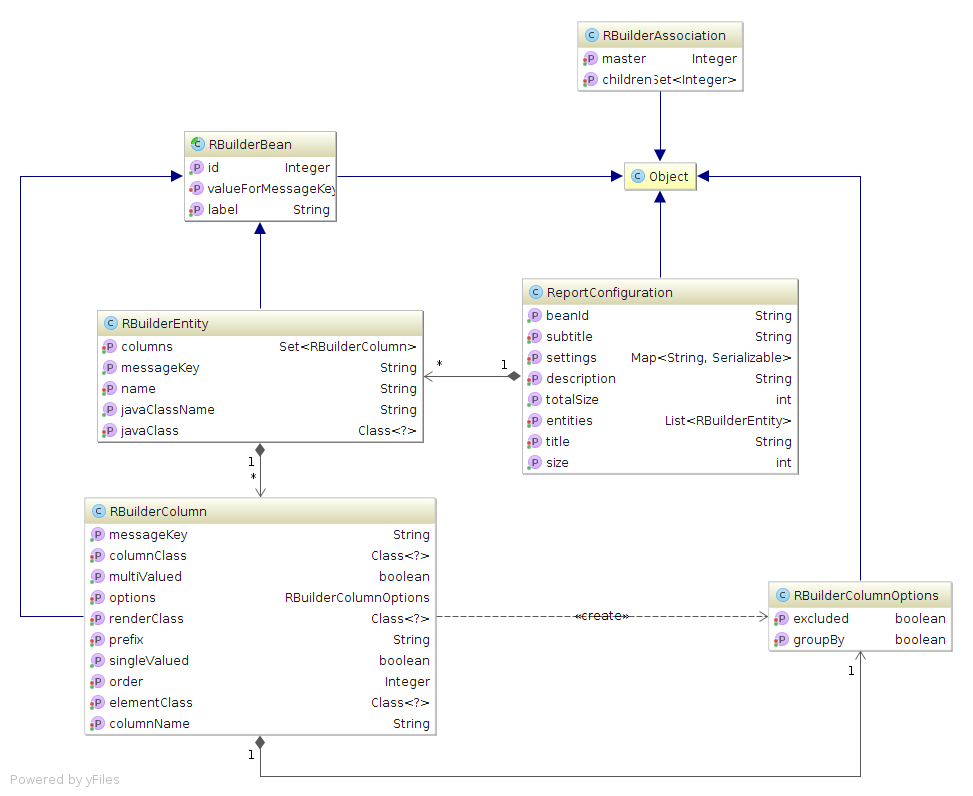
\includegraphics[width=1.0\textwidth]{images/rbuilder_dataModel}
				\caption[Diagram UML modelu danych \textbf{RBuilder}]{
					Diagram UML modelu danych \textbf{RBuilder}
				}
				\label{app:rbuilder_data_Model}
			\end{figure}	
			
			\paragraph{Serwisy}
			Serwisy \textbf{RBuilder}'a dostarczają metod dzięki którym możliwe jest wykonanie przygotowanie gotowego reportu
			w wybranej przez użytkownika reprezentacji, ale także utworzenie danych wymaganych przez kolejnego kroki przewodnika.
			Dostarczone usługi to:
			\begin{itemize}
				\item ustalenie możliwych typów w których można zrenderować wartość danej komórki / kolumny,
				\item tworzeniem obiektu domenowego w zależności od konfiguracji raportu,
				\item generowaniem instancji reprezentatywnego raportu
			\end{itemize}
			Funkcjonalność tej gruby klas do komponentu \textbf{RBuilder} można podzielić na następujące bloki:
			\begin{center}
				\begin{longtable}{| p{2.5cm} | p{13cm} |}
					\caption[Bloki funkcjonalne modelu serwisów \textbf{RBuilder}]{
						Bloki funkcjonalne modelu serwisów \textbf{RBuilder}			
					}\tabularnewline	
					
					\hline
						\multicolumn{1}{|c|}{\textbf{Grupa}} &
						\multicolumn{1}{|c|}{\textbf{Funkcjonalność}} \tabularnewline
					\hline
					\endfirsthead
					
					\multicolumn{2}{c}
					{{\bfseries \tablename\ \thetable{} -- kontynuacja...}} \tabularnewline
					\hline
						\multicolumn{1}{|c|}{\textbf{Grupa}} &
						\multicolumn{1}{|c|}{\textbf{Funkcjonalność}} \tabularnewline
					\hline
					\endhead
						
					\hline
						\multicolumn{2}{|r|}{{Następna strona...}} \tabularnewline \hline
					\endfoot
	
					\hline \hline
					\endlastfoot	
					
					\emph{Operation Management} 									& 
					Grupa \textbf{Operation Management} odpowiedzialna jest za instacjonowanie obiektu \textbf{SReport} w zależności
					od ilości wybranych dla konkretnego raportu. Lista klas:
					\begin{itemize}
						\item RBuilderOperation
						\item RBuilderCreateOperation
						\item SingleEntityRBuilderCreateOperation
						\item MultipleEntitiesRBuilderCreateOperation
					\end{itemize}					
					\hline
					\emph{Data Management}											&
					Klasy z grupy \textbf{Data Management} zostały zaprojektowane do pobierania danych takich jak:
					\begin{itemize}
						\item informacje o typach obiektów domenowych, które można uwzględnić w raportach. Takie klasy adnotowane są 
						przez adnotacje \emph{\@{}ReportableEntity}, a ich lista udostępniana jest poprzez interfejs \emph{ReportableEntityResolver},
						\item listę kolumn wraz z ich właściwościami takimi jak jej nazwą, nazwa dla wybranej lokalizacji językowej, typ danych
						przechowywanych w odpowiadającej jej polu w klasie, odpowiednie typu na które można rzutować dany typ. Informacje tego 
						typu udostępniane są poprzez interfejs \emph{ReportableBeanResolver},
						\item listą powiązań między modelami w uproszczonej formie na potrzeby wybierania tabel podczas projektowania raportu. 
						Na obecną chwile możliwe jest utworzenie jedynie nieprzechodnich powiązań opisanych na bazowym poziomie przez relacje
						klucz główny - obcy. Dane tego typu udostępnione są przez interfejs \emph{ReportableAssociationResolver}. 
					\end{itemize}
					\hline
					\emph{Dynamic Jasper Operation}								&
					\emph{JasperBuilderService} jest jedyną klasą tej grupy posiadającą dostarczającą możliwości utworzenia skompilowanego
					raportu typu \textbf{JasperReport}, który potem jest serializowany do systemu plików. Niemniej jego głównym zadaniem
					jest wkomponowanie w obiekty wyżej wymienionego typu takich danych jak:
					\begin{itemize}
						\item tytuł,
						\item podtytuł,
						\item opis,
						\item język,
						\item szerokość odpowiednich sekcji jak nagłówek, stopka itp.,
						\item lista kolumn,
						\item lista kolumn według których dane mają być grupowane.
					\end{itemize}
					\hline
					\emph{View helper}												&
					\emph{ReportBuilderService} jest interfejsem serwisu, którego celem istnienia jest przekazania sterowania do modułu
					\textbf{Operation Management} celem utworzenia instancji obiektu domenowego \textbf{SReport} oraz wsparcie
					dla operacji renderowania raportu w konkretnej reprezentacji. Kiedy pierwsza z funkcji jest trywialna w kontekście złożoności służąc
					jedynie separacji zadań i zmniejszeniu kohezji klas, druga z wymienionych metod jest dużo bardziej złożona.
					Jej celem jest wykonanie następujących operacji celem uzyskania danych wymaganych przez moduł \textbf{Spring} renderującego
					raport w wybranej reprezentacji (PDF, HTML, CSV, XLS):
					\begin{itemize}
						\item pobranie obiektu domenowego z bazy danych dla danego numeru raportu, 
						\item deserializacja skompilowanego pliku \textit{*.jasper} z systemu plików,
						\item utworzenie źródła danych na podstawie informacji takich jak lista kolumn, ich typ, wybranych typ reprezentacji danych w kolumnie
					\end{itemize}
					\hline
				\end{longtable}
				\label{app:rbuilder_services_functionality_table}
			\end{center}
						 
			\paragraph{Widok}
			Na tę część składają się następujące elementy:
			\begin{itemize}
				\item tabela z istniejącymi raportami \label{app:rbuilder_table},
				\item przewodnik tworzenia nowego raportu \label{app:rbuilder_wizard},
				\item specjalnie skonfigurowanego \textsc{ViewResolver}'a \footnote{\href{http://docs.spring.io/spring/docs/current/javadoc-api/org/springframework/web/servlet/ViewResolver.html}{ViewResolver} - interfejs, które implementują specjalne klasy zadaniem których jest ładowanie widoków poprzez odwołanie m.in. do plików JSP, logicznych nazw widoków itp.}.
			\end{itemize}

			Tabela (\ref{app:rbuilder_table}) jest obiektem należącym do warstwy widoku, który został utworzony z użyciem komponentu
			tabeli. Zawiera ona dodatkowo akcje, umożliwiające operacje na raportach. 
			% dodać IMG			
			
			Przewodnik (\ref{app:rbuilder_wizard}) został zaprojektowany na podstawie \textbf{Spring Web Flow}. Dzięki 
			temu zbiór formularzy, na których definiuje się poszczególne elementy składowe gotowego obiektu \textsc{ReportConfiguration}
			stanowiącego bazę do generowania wybranej reprezentacji \ref{app:rbuilder_representations} reportu, jest logicznie
			połączony. Dodatkową korzyścią jest uzyskanie bezproblemowego wsparcia dla przetwarzania uzyskanych danych wejściowych 
			po stronie serwera bez konieczności pisania własnej logiki do zarządzania komunikacją Ajax oraz możliwość przekazywania
			danych między kolejnymi krokami. 
			\begin{figure}[H]
				\centering
				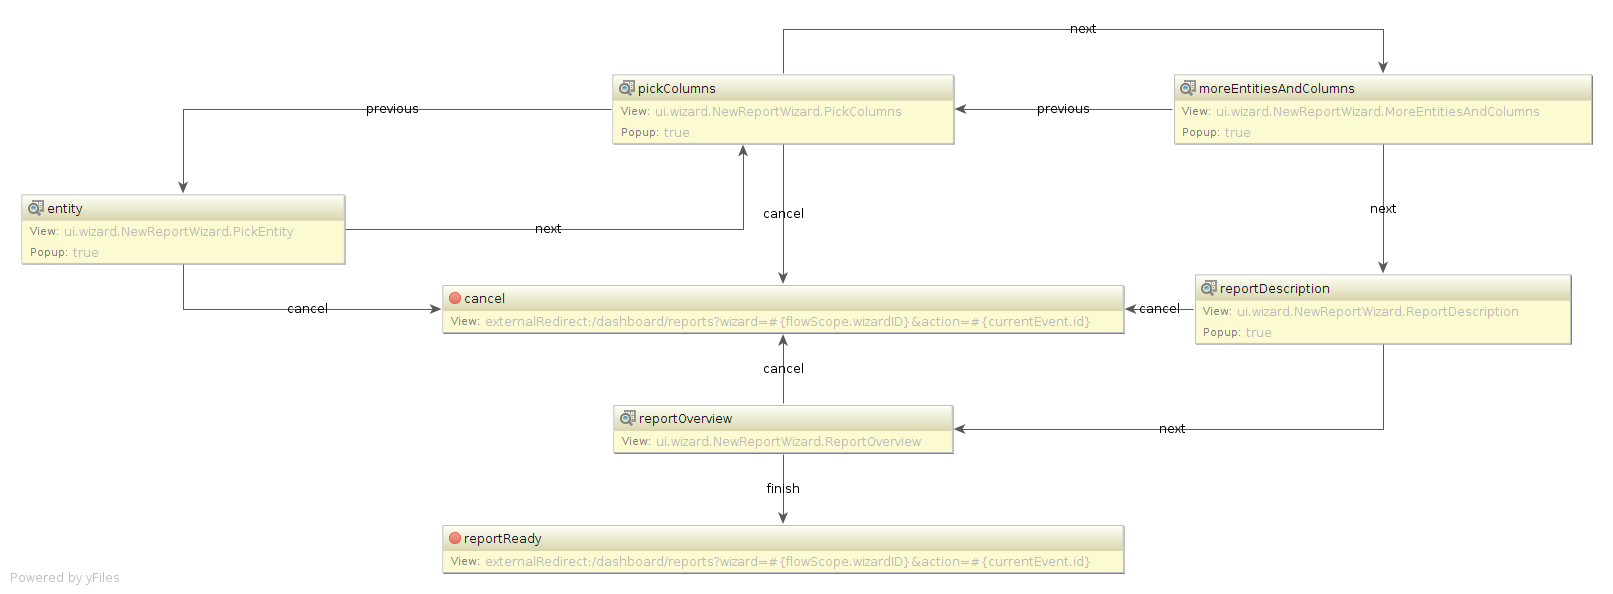
\includegraphics[width=1.0\textwidth]{images/rbuilder_flow}
				\caption[Logiczne połączenie kroków w przewodniku dla \textbf{RBuilder}]{
					Logiczne połączenie kroków w przewodniku dla \textbf{RBuilder}
				}
				\label{app:rbuilder_diagram_of_flow}
			\end{figure}
			Każdy z kroków przewodnika wspiera odpowiednia klasa Java będąca specjalizowanym rozszerzeniem \href{http://docs.spring.io/spring-webflow/docs/2.4.0.M1/api/org/springframework/webflow/action/FormAction.html}{FormAction} zarządzającą ustawieniem danych wejściowych
			dla formularza, walidacji i konwerterów. Ostatecznie rzecz jest szczególnie ważna ponieważ praktycznie wszystkie formularze
			zostały napisana aby wspierać wprowadzanie danych dla więcej niż jednego obiektu. Z uwagi na brak natywnego wsparcia ze strony
			szkieletu aplikacji \textbf{Spring} należało napisać odpowiednie metody samemu celem utworzenia z prostych łańcuchów
			znakowych poprawnych obiektów w danym kontekście. 
			\begin{code}
				\inputminted[
					lineos=true,
					firstline=151,
					lastline=169,
					fontfamily=monospace,
					obeytabs=true, 
					samepage=false,
					fontsize=\scriptsize
				]{java}{../../src/main/java/org/agatom/springatom/web/flows/wizards/wizard/rbuilder/PickEntityFormAction.java}
				% src file used
				\label{app:rbuilder_converter_of_data}
				\caption[Bazowy konwerter dla operacji \textbf{PickEntityFormAction}]{
					Bazowy konwerter dla operacji \textbf{PickEntityFormAction} który tworzy z łańcuchów
					znakowych obiekty \textbf{RBuilderEntity}
				}
			\end{code}
				 
		\subsubsection{Globalna - Warstwa konwersji}
			Warstwa konwersji typów jest modułem \textbf{Spring}, który wykorzystywany jest w momencie kiedy z obiektu typu
			A programista chce uzyskać obiekt typu B. Dobrym przykładem jest najczęściej moment w którym w kodzie JSP
			umieszczamy bezpośrednio nasz obiekt, korzystaj z biblioteki tagów dostarczonej przez \textbf{Spring}.
			W tym momencie uruchamiany jest proces mający na celu konwersję obiektu do reprezentatywnej postaci łańcucha znakowego,
			który można będzie wkomponować do drzewa DOM. 
			Jest to rozwiązanie efektywne niemniej posiadające jedno uchybienie. W przypadku gdy programista chciałby uzyskać
			selektywny sposób, zależny od kontekstu w jakim znajduje się obiekt lub też chęci uzyskania wartości
			jednego z atrybutów, nie jest on w stanie osiągnąć zamierzonego rezultatu z uwagi na sposób w jaki działa konwersja typów.
			Znalezienie pierwszego konwertera, który jest w stanie przeprowadzić żądaną transformację kończy proces wyszukiwania.
			Nie oznacza to wcale, że uzyskany wynik będzie zgodny z oczekiwanym. 
			Z tego powodu aplikacja demonstracyjna rozszerza istniejące funkcjonalność przez umożliwienie selektywnego
			konwertowania między poszczególnymi typami. Na obecną chwilę zostało to zaimplementowane dla obiektów domenowych, a
			klasą kontrolującą selektywny proces jest \textbf{PersistableConverterPicker}.
			\begin{code}
				\inputminted[
					lineos=true,
					firstline=43,
					lastline=105,
					fontfamily=monospace,
					obeytabs=true, 
					samepage=false,
					fontsize=\scriptsize
				]{java}{../../src/main/java/org/agatom/springatom/server/model/conversion/picker/PersistableConverterPicker.java}
				% src file used
				\label{app:conversion_persistableToString}
				\caption[\textbf{PersistableConverterPicker} - koordynator selektywnej konwersji typów]{
					\textbf{PersistableConverterPicker} - koordynator selektywnej konwersji typów
				}
			\end{code}
			\textbf{PersistableConverterPicker} posiada metody które pozwalają na wybór selektywnego konwertera do wykonania operacji
			transformacji. Zostało również zapewnione wsparcia dla istniejącej funkcjonalności, bez użycia selektora. Ta część realizowana jest w 
			metodzie \textbf{PersistableConverterPicker\#{}getDefaultConverter(...)}. Selektywne konwertery różnią się od normalnych jedynie
			użyciem specjalnej adnotacji, która pozwala na ustalenie, że:
			\begin{itemize}
				\item konwerter jest domyślny jeśli nie został zdefiniowany klucz,
				\item konwerter jest selektywny jeśli istnieje zdefiniowany klucz.
			\end{itemize}
		
	\subsection{Plany rozwojowe}
	Aplikacja demonstracyjna jest obecnie na etapie dalszego rozwoju. Posiada szeroko zdefiniowane modułu zaprojektowane aby wspierać takie
	rejony jak:
	\begin{itemize}
		\item generyczna warstwa operacji bazodanowych,
		\item warstwa logiki biznesowej udostępnionej przez serwisy,
		\item moduł komponentów dla budowy tabel oraz stron obiektów domenowych,
		\item selektywna warstwa konwersji,
		\item tagi oddelegowane dla przewodników opartych o Spring Web Flow,
		\item model danych wraz z jego abstrakcyjną warstwą (interfejsy) do użytku zewnętrznego,
		\item moduł obsługujący funkcjonalność raportowania 
	\end{itemize}
	W większości przypadków uzyskana funkcjonalność jest jednak na etapie implementacji i niektóre z niedopracowanych elementów 
	ulegną zmianie celem uproszczenia zarządzaniem złożonością projektu oraz usunięciem nadmiarowych klas oraz słabo
	konfigurowalnych części.
	Plany rozwojowe aplikacji zostały zestawione w poniższej tabeli.
	\begin{center}
		\begin{longtable}{|l|l|p{10cm}|}
			\caption[Plany rozwojowe aplikacji demonstracyjnej]{
				Plany rozwojowe aplikacji demonstracyjnej
			}\tabularnewline	
			
			\hline
				\multicolumn{1}{|c|}{\textbf{LP}} 			&
				\multicolumn{1}{|c|}{\textbf{Moduł}}		&
				\multicolumn{1}{|c|}{\textbf{Opis zmian}}	\tabularnewline
			\hline
			\endfirsthead
			
			\multicolumn{2}{c}
			{{\bfseries \tablename\ \thetable{} -- kontynuacja...}} \tabularnewline
			\hline
				\multicolumn{1}{|c|}{\textbf{LP}} 			&
				\multicolumn{1}{|c|}{\textbf{Moduł}}		&
				\multicolumn{1}{|c|}{\textbf{Opis zmian}}	\tabularnewline
			\hline
			\endhead
				
			\hline
				\multicolumn{2}{|r|}{{Następna strona...}} \tabularnewline \hline
			\endfoot

				\hline \hline
			\endlastfoot	
			
			\emph{1}					&
			\textbf{ComponentBuilder}	&
			\begin{itemize}
				\item optymalizacja kodu oraz wsparcie dla cache'owania raz załadowanych
				\item przeniesienie definicji stron do deklaratywnego języka XML.
				Będzie to możliwe po usprawnieniu działania selektywnych konwerterów oraz 
				zwiększy możliwość zmian zgodnie z wymaganiami bez konieczności zmian w plikach Java,
				\item prawdopodobne przeprojektowanie operacji ładowania 
				strony obiektu domenowego. Na obecną chwilę ładowany jest gotowy widok,
				jednakże z uwagi na możliwie duży narzut 
				przesłanych danych bardziej optymalnym rozwiązaniem jest załadowanie pojedynczo 
				każdego z panelu zdefiniowanego na danej stronie,
				\item przeniesienie kodu widoku stron domenowych do łatwiejszego w zarządzaniu oraz utrzymaniu kodu ExtJS
			\end{itemize}
										\tabularnewline
										
			\emph{2}					&
			\textbf{ComponentBuilder}	&
			Połączenie kontrolerów odpowiedzialnych 
			za obsługę żądań pochodzących od komponentów typu \textbf{tabele} oraz \textbf{strony domenowe}. 
			Celem tego działania jest ujednolicenie 
			adresów sugerujące, że oba moduły wywodzące się z tej samej rodziny klas oraz służą podobnemu
			celowi. Oddelegowania właściwego uzyskania 
			wyniku zarówno w kwestii danych jak i definicji przez oddelegowane klasy. 
										\tabularnewline
										
			\emph{3}					&
			\textbf{ComponentBuilder}	&
			Wprowadzenie automatycznego mechanizmu generującego przekierowania do stron obiektów domenowych
										\tabularnewline
										
			\emph{4}					&
			\textbf{WebFlow}			&
			Zaprojektowanie biblioteki wspierającej 
			funkcjonalność \textbf{Spring Web Flow} dla biblioteki ExtJS. Decyzja podyktowana jest 
			chęcią zminimalizowania użycia różnorodnych bibliotek JavaScript. Gotowa biblioteka
			byłaby udostępniona na licencji OpenSource.
										\tabularnewline
			\emph{5}						&
			\textbf{Selektywne konwertery}	&
			Rozszerzenie możliwości selektywnych konwerterów o obiekty inne niż domenowego oraz
			wsparcie dla możliwości definiowana powtarzających się selektorów - kluczy w kontekście
			globalnym, ale unikatowych w kontekście danego obiektu podlegającego konwersji.
										\tabularnewline
			\emph{6}						&
			\textbf{Kod ogólny}				&
			Usunięcie pozostałości nadmiarowego kodu, który pozostał po uaktualnieniu aplikacji
			do korzystania z najnowszej (4.0.0) wersji szkieletu aplikacji Spring. Dzięki wprowadzonym 
			poprawkom oraz nowym funkcjom część istniejącego kodu możliwa będzie do zastąpienie
			przez kod szkieletu co zmniejszy stopień bezpośredniej zależności między aplikacją a framework'iem.
											\tabularnewline
			\emph{7}						&
			\textbf{Widok}					&
			Wsparcia dla ExtJS - migracja istniejących komponentów warstwy widoku użytkownika do 
			szkieletu aplikacji ExtJS. Prawdopodobnym wyborem będzie wykorzystanie ExtJS w wersji 4.x.x z uwagi
			na lepszą wydajność i większe możliwości biblioteki. 
											\tabularnewline
			\emph{8}						&
			\textbf{ReportBuilder}			&
			Zrezygnowania z ciężkiego w użyciu oraz utrzymaniu sposobu generowania raportów w aplikacji poprzez
			bibliotekę \textbf{DynamicJasper}. Przeniesienie bezpośredniego generowania raportów do tabelek oraz
			inwestygacja możliwych technologii do wykorzystania w przypadku eksportowania raportu do formatów takich jak
			HTML, CSV, PDF oraz XLS.		
											\tabularnewline		
			\emph{9}						&
			\textbf{Wizard'y}				&
			Ukończenie wszystkich wymaganych kreatorów zarówno modyfikacja jak i tworzenia nowych obiektów domenowych	
											\tabularnewline	
			\emph{10}						&
			\textbf{Terminarz spotkań}		&
			Ukończenie prac nad terminarzem spotkań. Obecna funkcjonalność pozwala na tworzenie obiektów, które następnie
			można przeglądać z użyciem kalendarza (podobny do używanego w programie Outlook). 	
											\tabularnewline								
		\end{longtable}
		\label{app:changes_in_future}
	\end{center}
		
\section{Diagramy UML, schemat bazy danych}
	\subsection{Schemat bazy danych}
	\begin{figure}[H]
		\centering
		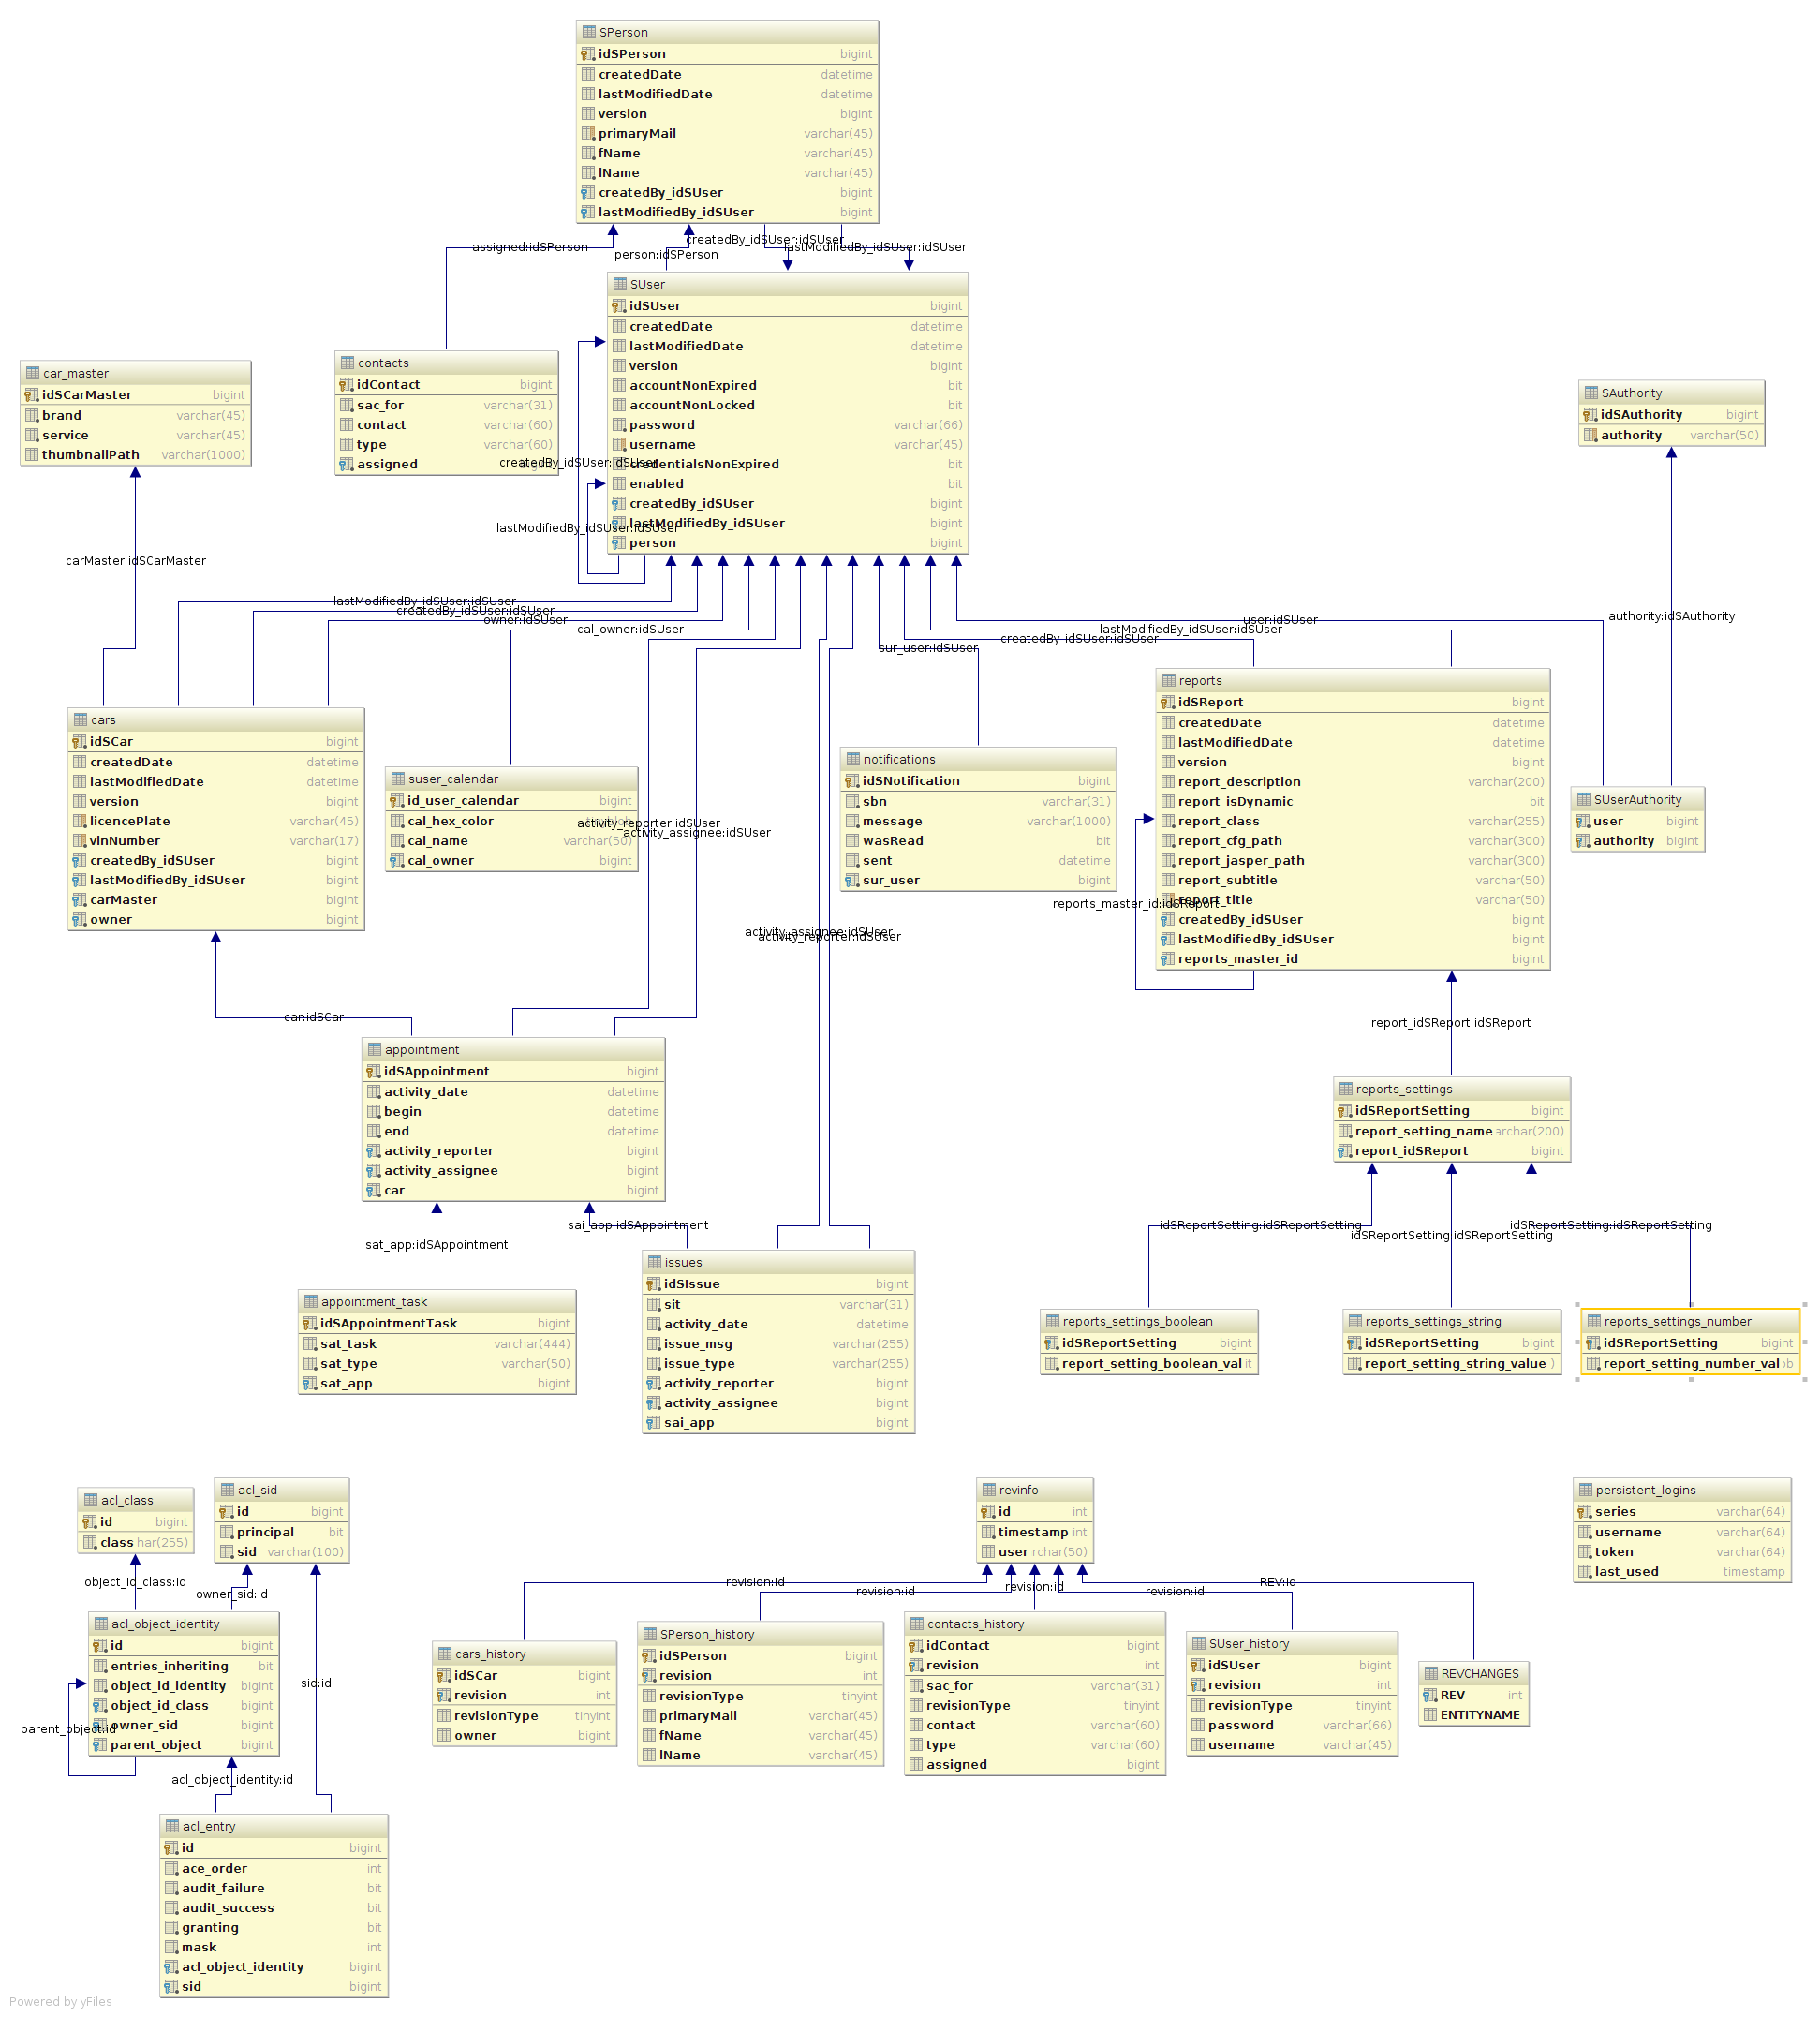
\includegraphics[width=1.1\textwidth]{images/db_UML}
		\caption[Schemat bazy danych aplikacji demonstracyjnej]{
			Schemat bazy danych aplikacji demonstracyjnej
		}
		\label{app:schema_db}
	\end{figure}
	\begin{figure}[H]
		\centering
		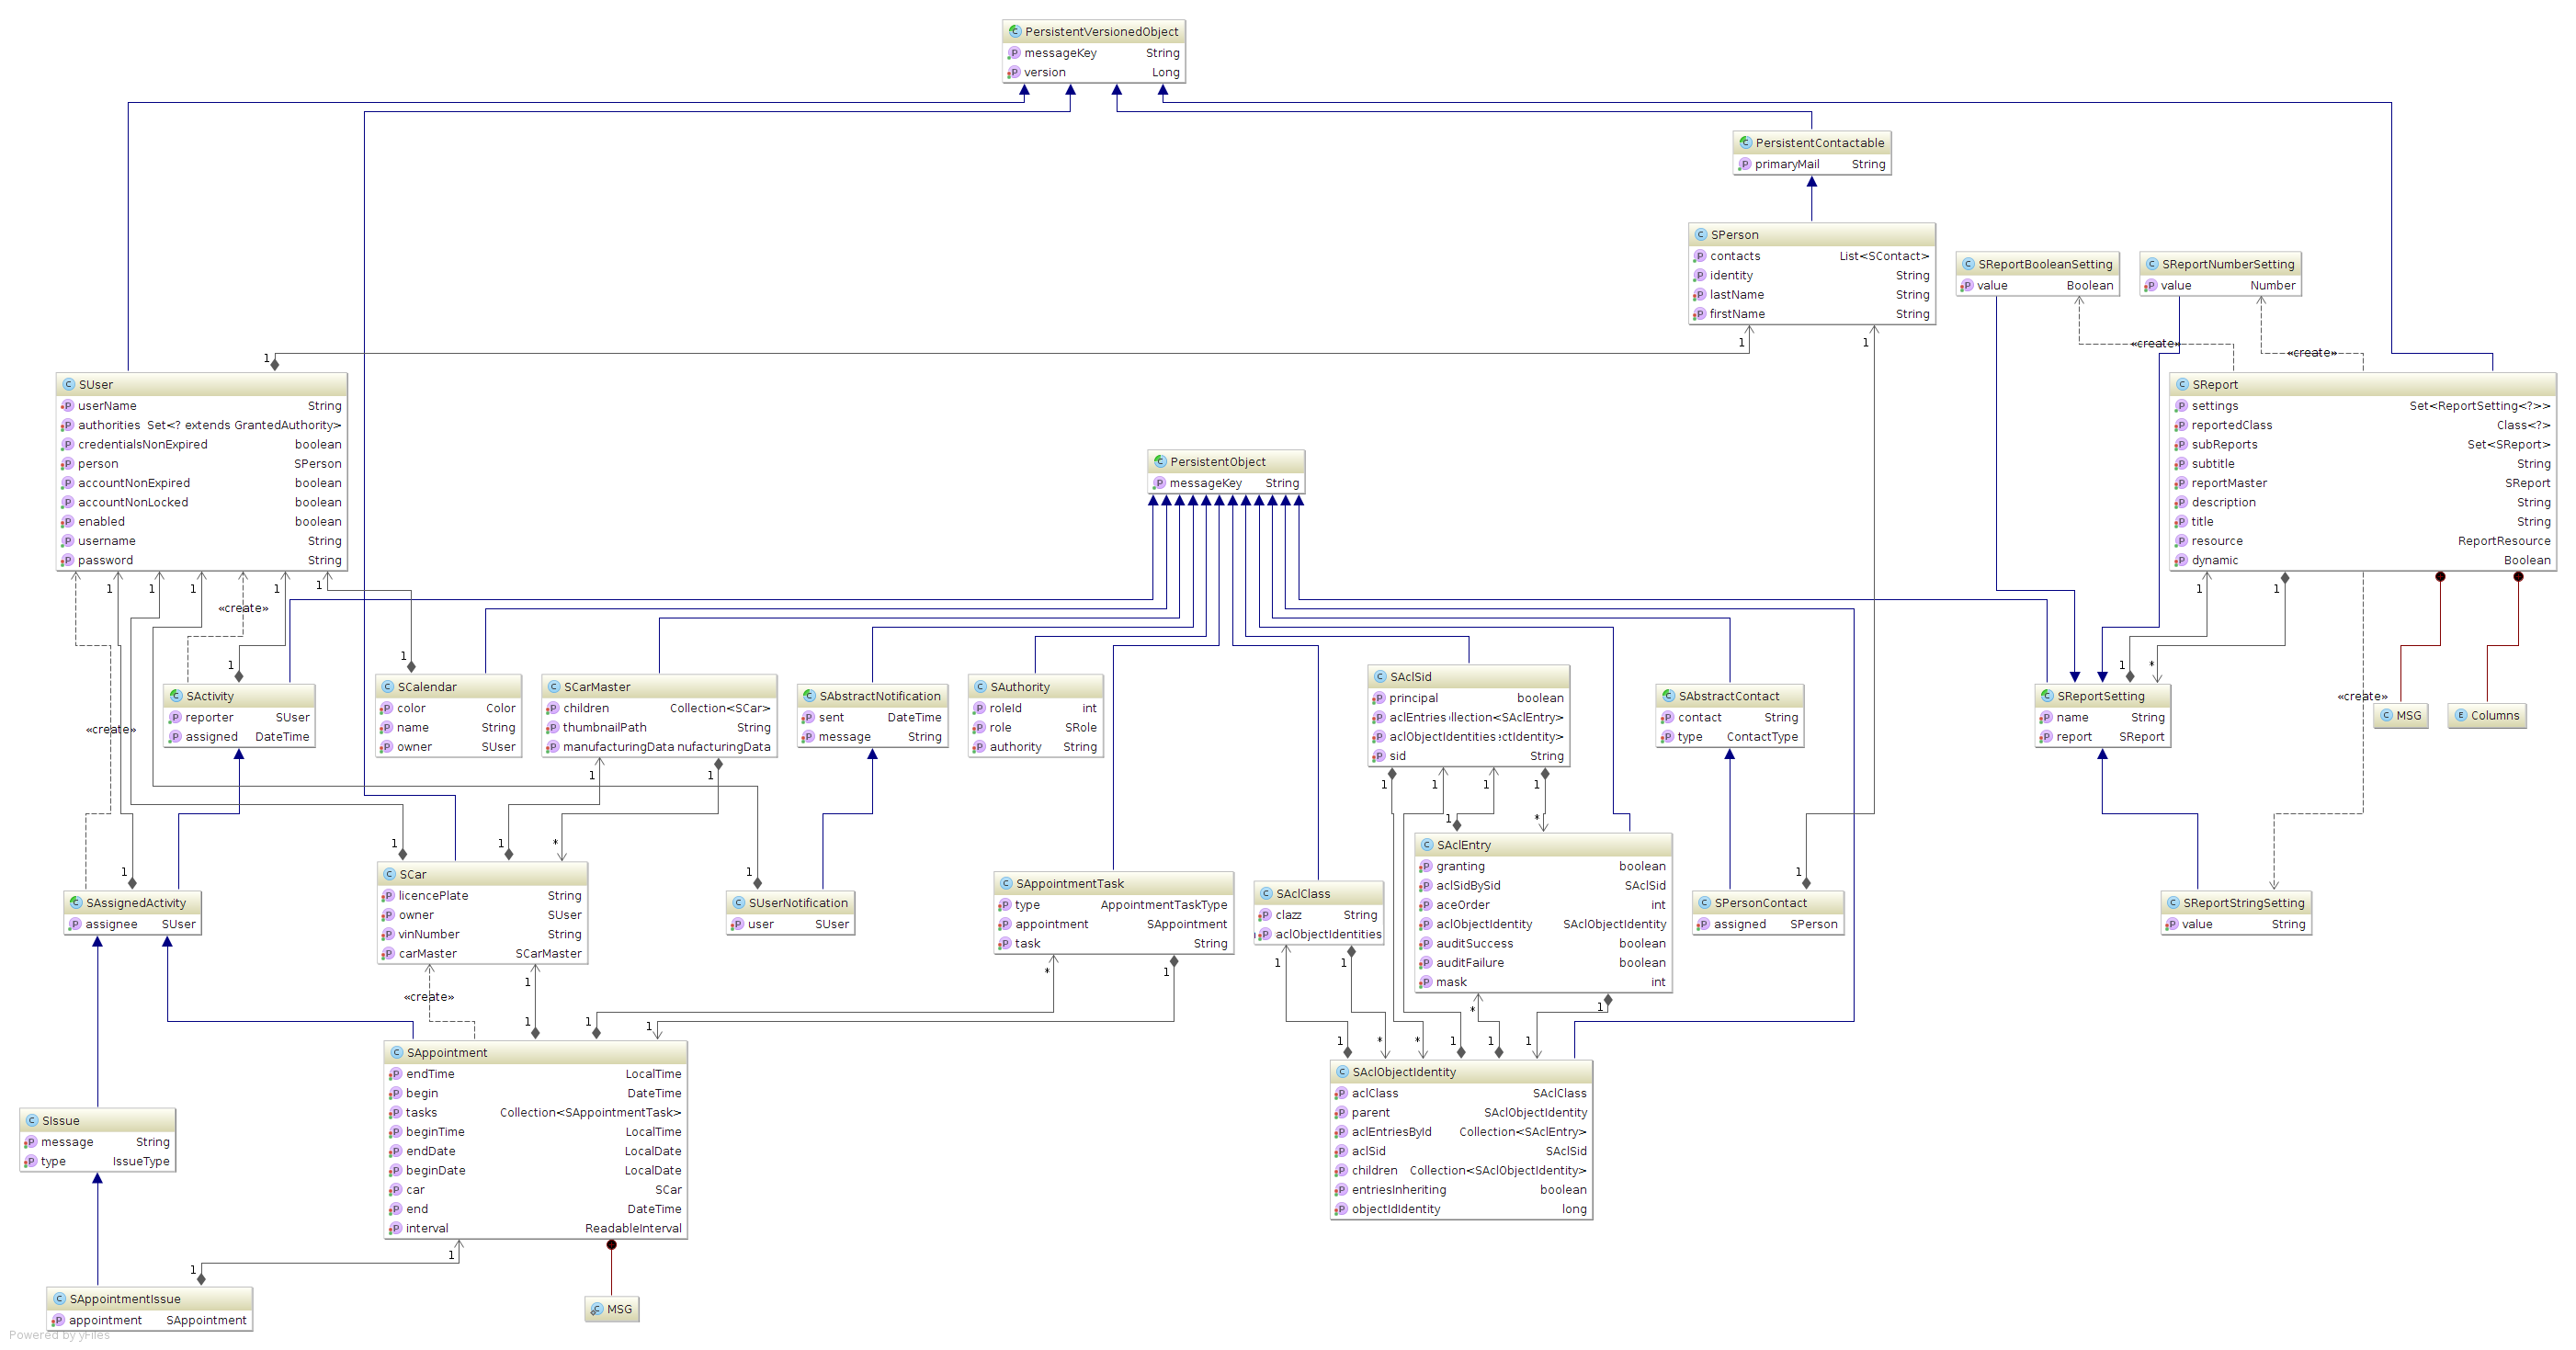
\includegraphics[angle=90,height=\textheight]{images/springatom_model_uml}
		\caption[Obiektowy model danych]{
			Obiektowy model danych odpowiadający\\który odpowiada schematowi bazy danych
		}
		\label{app:schema_org_agatom_springatom_model}
	\end{figure}
	\begin{figure}[H]
		\centering
		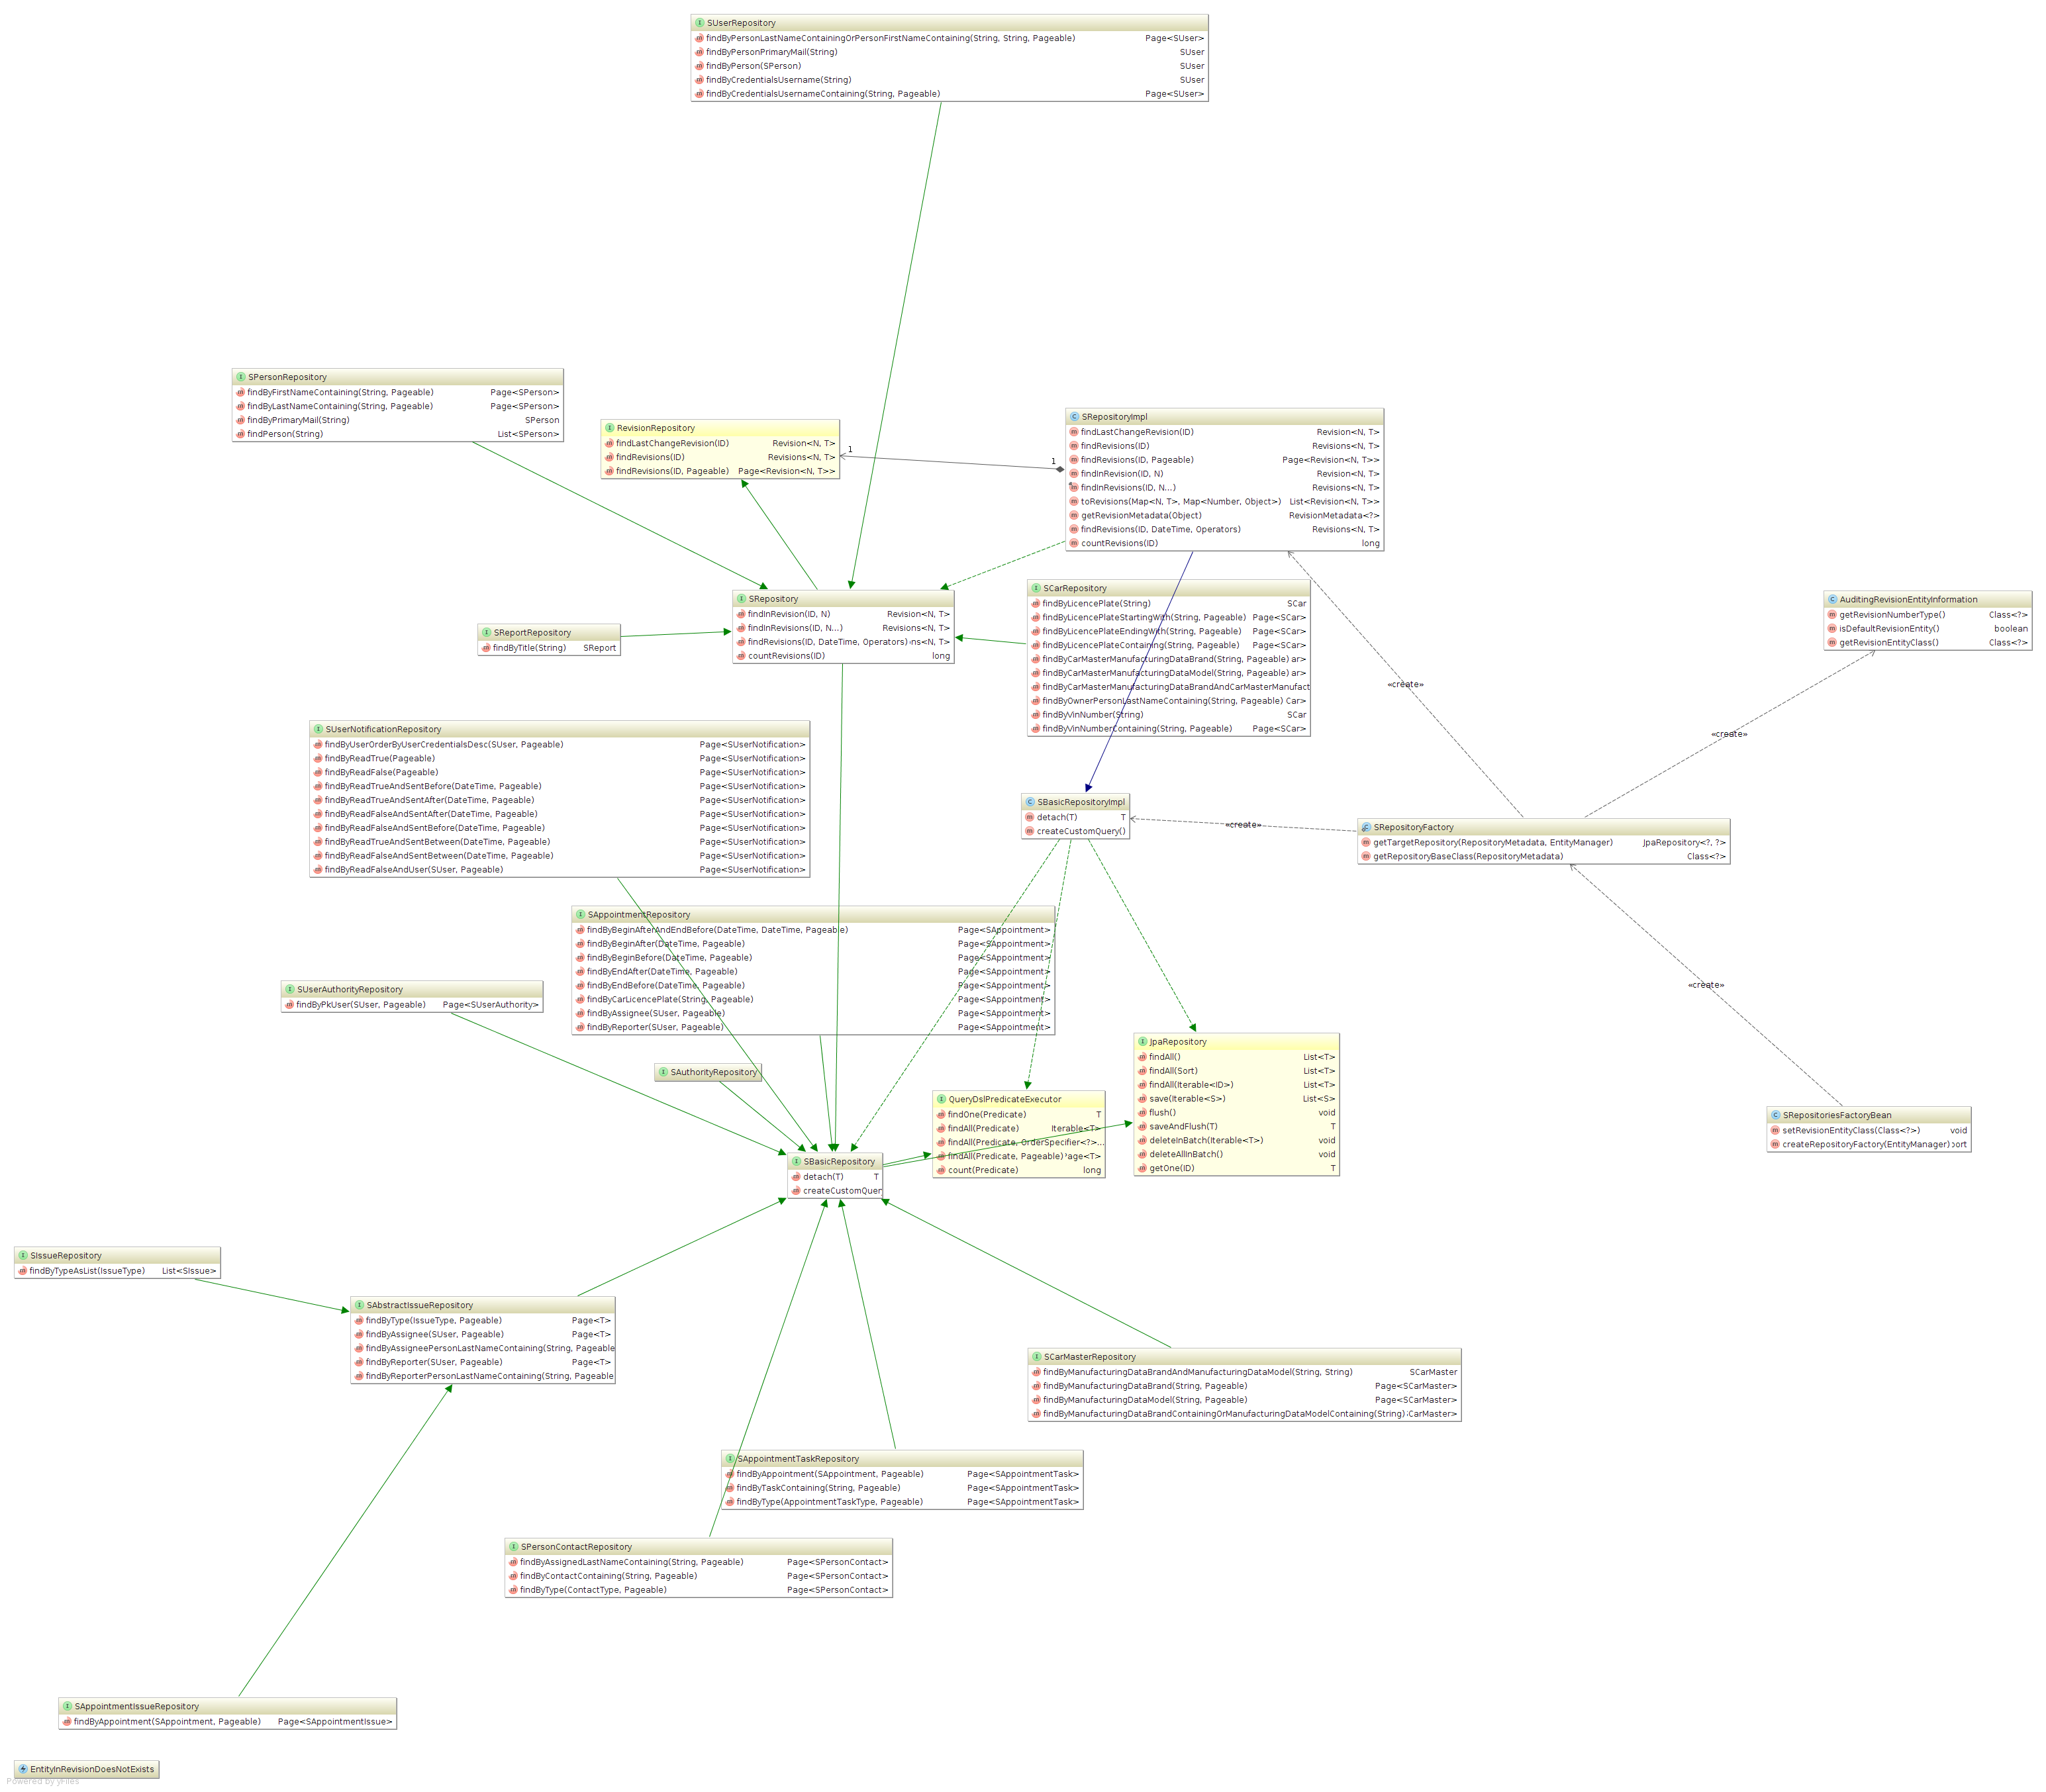
\includegraphics[width=\textwidth]{images/springatom_model_repository}
		\caption[Schemat repozytoriów aplikacji demonstracyjnej]{
			Schemat repozytoriów aplikacji demonstracyjnej
		}
		\label{app:schema_org_agatom_springatom_repository}
	\end{figure}
	
	\todo[inline]{Add the rest of UMLs}
		
\section{Metryki kodu}
	Kod aplikacji jest zbiorem funkcjonalności zaimplementowanych zarówno dla części serwerowej jak i klienckiej. Z tego powodu liczba linii kodu
	została podzielona na odpowiednie grupy zgodne z językami użytymi do stworzenia aplikacji demonstracyjnej.
	\subsection{Liczba linii kodu aplikacji}
	\begin{center}
		\begin{longtable}{|l|l|l|l|l|}
			\caption[Liczba linii kodu według języka programowania]{
				Liczba linii kodu według języka programowania
			}\tabularnewline	
			
			\hline
				\multicolumn{1}{|c|}{\textbf{Język}} 			&
				\multicolumn{1}{|c|}{\textbf{LOC}} 			&
				\multicolumn{1}{|c|}{\textbf{LOC (SC)}} 		&
				\multicolumn{1}{|c|}{\textbf{LOC (C)}} 		&
				\multicolumn{1}{|c|}{\textbf{LOC (EL)}} 		\tabularnewline
			\hline
			\endfirsthead
			
			\multicolumn{2}{c}
			{{\bfseries \tablename\ \thetable{} -- kontynuacja...}} \tabularnewline
			\hline
				\multicolumn{1}{|c|}{\textbf{Język}} 			&
				\multicolumn{1}{|c|}{\textbf{LOC}} 			&
				\multicolumn{1}{|c|}{\textbf{LOC (SC)}} 		&
				\multicolumn{1}{|c|}{\textbf{LOC (C)}} 		&
				\multicolumn{1}{|c|}{\textbf{LOC (EL)}} 		\tabularnewline
			\hline
			\endhead
				
			\hline
				\multicolumn{2}{|r|}{{Następna strona...}} \tabularnewline \hline
			\endfoot

				\hline \hline
			\endlastfoot	
			
			\emph{Java}		& 29555	 	& 16628 	& 9136 		& 3791 	\hline
			\emph{JS} 		& 1044	 	& ? 		& ? 		& ? 	\hline
			\emph{JSP} 		& 2122	 	& ? 		& ? 		& ? 	\hline
			\emph{Razem} 	& 32721	 	& 16628 	& 9136 		& 3791  \hline
		\end{longtable}
		\label{app:code_metric_loc}
		\begin{tabular}{l l}
				LOC 		& Całkowita liczba linii kodu 	\\
				LOC (SC)	& Liczba linii kodu źródłowego \\
				LOC (C)		& Liczba linii komentarzy		\\
				LOC (EL)	& Liczba linii pustych
		\end{tabular}	
	\end{center}
	
	\subsection{Java}
	Zadaniem tabel \ref{app:code_metric_loc} (dodać resztę) jest zobrazowanie złożoności projektu, którego celem prócz dostarczenie finalnej funkcjonalności, jest zaprojektowanie
	kilku modułów do późniejszej publikacji oraz wykorzystania w innych projektach. Projekt składa się z 5 głównych modułów:
	\begin{itemize}
		\item \textbf{AOP} - funkcjonalność opierająca się o \textit{Aspect Oriented Programming}, działająca globalnie na całą aplikację i wspomagające niektóre z funkcjonalności,
		bez konieczności implementacji metod w konkretnych metod lub wykorzystywaniu statycznych metod różnych klas pomocniczych. Działanie klas tego modułu jest wysoce transparentne
		a funkcje wykorzystywane i odsperarowane od reszty aplikacji są wykonywane wspierając ją. Niemniej jest pewna znacząca różnica. Nie ma potrzeby bezpośrednio wprowadzania 
		zależności między klasami wykorzystujący programowanie aspektowe a klasami objętymi ich działanie,
		\item \textbf{Core} - zbiór artefaktów (klas, klas abstrakcyjnych, interfejsów oraz typów wyliczeniowych) przeznaczonych do wykorzystanie w innych miejscach aplikacji celem
		dostarczenie właściwej funkcjonalności,
		\item \textbf{Server} - zadaniem klas tego modułu jest dostarczenie modelu danych, wsparcia jego walidacji oraz wersjonowania, definicje interfejsów repozytoriów oraz serwisów odpowiedzialnych
		za logikę biznesową oraz funkcjonalność dla operacji na plikach XML. 
		\item \textbf{Web} - artefakty tego modułu stanowią zbiór zarówno klas wspomagających funkcjonalność warstwy MVC (wszelakiego rodzaju modelowania akcji dla warstwy widoku, pełna definicja
		modułu komponentów, definicje tagów wspierających przewodniki definiowane na bazie \textbf{Spring Web Flow}, moduł raportowania, czy też ostatecznie wszelakiego rodzaju klasy pomocnicze
		przeznaczone dla tak zwanych \textit{interceptor}'ów\footnote{Interceptor - specjalne klasy które można wpiąć w dowolny etap wywołania danego widoku po adresie URI celem wprowadzenia
		danych bądź zmiennych}.
		\item \textbf{WebMVC} - zbiór wszelakich artefaktów przeznaczonych do implementacji warstwy MVC. W zbiorze artefaktów tego modułu znajdują się między innymi kontrolery, konwertery danych,
		wspomniane już wcześniej \textit{interceptor}'y (korzystające z klas zdefiniowanych w modelu \textbf{Web} celem dostarczania danych dla widoków, definicje klas zajmujących się dostarczaniem
		definicji oraz danych dla komponentów takich jak tabele i strony domenowe obiektów.
	\end{itemize}	
	\subsubsection{Strukturalne metryki kodu}
	\begin{center}
		\begin{longtable}{|l|l|l|l|l|l|}
			\caption[Liczba klas / Liczba linii kodu modułów]{
				Liczba klas / Liczba linii kodu modułów	
			}\tabularnewline	
			
			\hline
				\multicolumn{1}{|c|}{\textbf{Moduł}} 			&
				\multicolumn{1}{|c|}{\textbf{LK}} 				&			
				\multicolumn{1}{|c|}{\textbf{LOC}}				&		
				\multicolumn{1}{|c|}{\textbf{CD}}				&	
				\multicolumn{1}{|c|}{\textbf{D}}				&
				\multicolumn{1}{|c|}{\textbf{TD}}				
				\tabularnewline
			\hline
			\endfirsthead
			
			\multicolumn{2}{c}
			{{\bfseries \tablename\ \thetable{} -- kontynuacja...}} \tabularnewline
			\hline
				\multicolumn{1}{|c|}{\textbf{Moduł}} 			&
				\multicolumn{1}{|c|}{\textbf{LK}} 				&			
				\multicolumn{1}{|c|}{\textbf{LOC}}				&		
				\multicolumn{1}{|c|}{\textbf{CD}}				&	
				\multicolumn{1}{|c|}{\textbf{D}}				&
				\multicolumn{1}{|c|}{\textbf{TD}}					
				\tabularnewline
			\hline
			\endhead
				
			\hline
				\multicolumn{2}{|r|}{{Następna strona...}} \tabularnewline \hline
			\endfoot

				\hline \hline
			\endlastfoot	
			
			\emph{Aop}			&  3/3			& 	192/192			& 	0		& 	0		&	0		\hline
			\emph{Core}			&  13/1.86		& 	628/89.71		&	0		&	0.25	&	0.25	\hline
			\emph{Server}		&  187/3.07		& 	10806/183.15	&	0.82	&	3.32	&	23.48	\hline
			\emph{Web}			&  188/2.89		& 	10803/166.20	&	0.3		&	3.28	&	14.01	\hline
			\emph{WebMVC}		&  37/2.85		& 	2262/174		&	0		&	4.27	&	37.73	\hline
		\end{longtable}
		\label{app:modules_code_metrics}		
		\begin{tabular}{l l}
				LK 		& 	Liczba klas/Średnia liczba klas				\\
				LOC		& 	Liczba linii kodu/Średnia liczba linii kodu	\\
				D		& 	Średnia liczba cyklicznych zależności			\\
				CD		& 	Średnia liczba zależności						\\
				TD		& 	Średnia liczba zależności przechodnich			\\
		\end{tabular}	
	\end{center}
	
	\subsubsection{Metryka Chidamber & Kemerer}
	Zadaniem metryki jest analiza następujących metryk kodu \cite{chidamberKemerer}:
	\begin{itemize}
		\item \textbf{WMC} - liczba metod zdefiniowanych w klasie,
		\item \textbf{DIT} - głębokość drzewa dziedziczenia,
		\item \textbf{SUB} - liczba bezpośrednich potomków w hierarchii dziedziczenia,
		\item \textbf{CBO} - stopień zależności od pozostałych artefaktów,
		\item \textbf{RFC} - responsywność klasy, czyli możliwość jej odpowiedzi na wywołania przez inne obiekty innych klas,
		\item \textbf{LCOM} - stopień kohezji, im wyższy oznacza większą zależność między poszczególnymi elementami
	\end{itemize}
	
	\begin{center}
		\begin{longtable}{|l|l|l|l|l|l|l|}
			\caption[Metryka Chidamber - Kemerer]{
				Metryka Chidamber - Kemerer	
			}\tabularnewline	
			
			\hline
				\multicolumn{1}{|c|}{\textbf{Moduł}} 			&
				\multicolumn{1}{|c|}{\textbf{CBO}}				&		
				\multicolumn{1}{|c|}{\textbf{DIT}}				&	
				\multicolumn{1}{|c|}{\textbf{LCOM}}			&
				\multicolumn{1}{|c|}{\textbf{RFC}}				&	
				\multicolumn{1}{|c|}{\textbf{SUB}}				&
				\multicolumn{1}{|c|}{\textbf{WMC}} 			\tabularnewline
			\hline
			\endfirsthead
			
			\multicolumn{2}{c}
			{{\bfseries \tablename\ \thetable{} -- kontynuacja...}} \tabularnewline
			\hline
				\multicolumn{1}{|c|}{\textbf{Moduł}} 			&
				\multicolumn{1}{|c|}{\textbf{CBO}}				&		
				\multicolumn{1}{|c|}{\textbf{DIT}}				&	
				\multicolumn{1}{|c|}{\textbf{LCOM}}			&
				\multicolumn{1}{|c|}{\textbf{RFC}}				&	
				\multicolumn{1}{|c|}{\textbf{SUB}}				&
				\multicolumn{1}{|c|}{\textbf{WMC}} 			\tabularnewline
			\hline
			\endhead
				
			\hline
				\multicolumn{2}{|r|}{{Następna strona...}} \tabularnewline \hline
			\endfoot
				\hline \hline
			\endlastfoot	
			
			\emph{Aop}			&  0		& 	1.00	& 	2.33	& 	12.00	&	0		&	6		\hline
			\emph{Core}			&  2.25		& 	1.50	&	1.00	&	34.60	&	0.62	&	5.12	\hline
			\emph{Server}		&  6.50		& 	2.35	&	1.64	&	282.30	&	0.77	&	7.16	\hline
			\emph{Web}			&  5.78		& 	2.03	&	1.74	&	194.33	&	0.64	&	7.47	\hline
			\emph{WebMVC}		&  5.00		& 	2.94	&	1.33	&	213.22	&	0.18	&	5.03	\hline
			\emph{Razem}		&  5.78		&	2.22	&	1.65	&	222.44	&	0.62	&	6.98	\hline
		\end{longtable}
		\label{app:chidamberKemerer}
	\end{center}
	
	Na uwagę zasługują w tym miejscu niskie wartości takich współczynników 
	jak \textbf{DIT} gdzie średnia wartość nie przekroczyła wartości 3 począwszy
	od korzenia wszystkich klas definiowanych w języku Java - \textbf{Object}. 
	Przyjmuje się, że wartość graniczna dla większości aplikacji wynosi 5.
	Niemniej wartość średnia nie oddaje pojedynczych przypadków nadużyć. 
	Większość przypadków występujących  aplikacji demonstracyjnej, które
	przekraczają graniczną wartość, odnosi się do klas rozszerzających 
	standardowe możliwości szkieletu aplikacji celem dostosowania ich do konkretnych przypadków użycia.
	Dzieje się tak w przypadku wprowadzanie wsparcia dla biblioteki \textbf{Apache Tiles 3} 
	dla częściowego ładowania stron w szczególni dla modułów opierających się na
	\textbf{Spring Web Flow}. Inną grupą przypadków jest głębokość dziedziczenia 
	przekraczająca przyjętą wartość w klasach opisujących biznesowy model danych. Fakt ten można
	pominąć z uwagi na to, że wspomniane artefakty służą wsparciu dla dziedziczenia 
	wspólnych atrybut dla konkretnych gałęzi klas oraz tym, że są to w klasy definiujące, prócz 
	wspomnianych już pól, metody dostępowe takie jak popularnie nazywane \textbf{gettery} 
	oraz \textbf{settery}. W nielicznych przypadkach część funkcjonalności biznesowej została
	zamknięta w obiektach domenowych z uwagi na rozbieżność w sposobie przechowywania 
	danych a typami jakie są udostępnienie zewnętrznym klasom. 
	
	W tym miejscu warto nadmienić o wartości jaką uzyskano dla wskaźnika \textbf{SUB}, 
	który jest blisko związany z poprzednio omawianym \textbf{DIT}. 
	Podczas gdy \textbf{DIT} opisuje głębokość drzewa dziedziczenia, 
	co przekłada się na zwiększenie zarówno ilości atrybut jak i metod będących
	kandydatami do ponownego wykorzystania (nadpisania), \textbf{SUP} 
	odnosi się do szerokości drzewa dziedziczenia, czyli ilości dzieci będących 
	bezpośrednimi potomkami analizowanej klasy. Przyjęto, że niska wartość 
	\textbf{DIT} jest zdecydowania lepsza od \textbf{SUB}. Tak też jest w przypadku aplikacji
	demonstracyjnej, gdzie wartości tych dwóch współczynników 
	charakteryzują się następującymi wartościami \textbf{DIT=2.22} oraz \textbf{SUB=0.62}. Widać wyraźnie, że
	zdecydowana większość klas definiuje swoją rolę poprzez mechanizm polimorfizmu.
	
	Największym problem aplikacji okazała się wysoka wartość 
	współczynnika \textbf{RFC}. Im jest ona wyższa tym bardziej aplikacja narażona jest na błędy, a
	istniejąca złożoność utrudnia zrozumienie oraz testowanie aplikacji. 
	
	\subsubsection{Metryka MOOD}
	Zadaniem metryk \textbf{MOOD} zostały zaprojektowane do mierzenia globalnej jakości projektu OOP\cite{moodMetrics}.
	Analiza projektu tymi metrykami jest szczelnie użyteczna dla dużych projektów zaprojektowanych z użyciem technik 
	programowania obiektowego. Duża ilość klas projektu oraz istniejące na tym etapie plany rozwojowego sugerujące dalszy
	wzrost ilości linii kodu sprawiają, że powyższe analizy stanowią dobry wybór. 
	\begin{center}
		\begin{longtable}{|l|l|l|l|l|l|l|}
			\caption[Metryka MOOD]{Metryka MOOD}
			\tabularnewline	
			
			\hline
				\multicolumn{1}{|c|}{\textbf{Projekt}} 			&
				\multicolumn{1}{|c|}{\textbf{AHF}}				&		
				\multicolumn{1}{|c|}{\textbf{AIF}}				&	
				\multicolumn{1}{|c|}{\textbf{CF}}				&
				\multicolumn{1}{|c|}{\textbf{MHF}}				&	
				\multicolumn{1}{|c|}{\textbf{MIF}}				&
				\multicolumn{1}{|c|}{\textbf{PF}} 				\tabularnewline
			\hline
			\endfirsthead
			
			\multicolumn{2}{c}
			{{\bfseries \tablename\ \thetable{} -- kontynuacja...}} \tabularnewline
			\hline
				\multicolumn{1}{|c|}{\textbf{Projekt}} 			&
				\multicolumn{1}{|c|}{\textbf{AHF}}				&		
				\multicolumn{1}{|c|}{\textbf{AIF}}				&	
				\multicolumn{1}{|c|}{\textbf{CF}}				&
				\multicolumn{1}{|c|}{\textbf{MHF}}				&	
				\multicolumn{1}{|c|}{\textbf{MIF}}				&
				\multicolumn{1}{|c|}{\textbf{PF}} 				\tabularnewline
			\hline
			\endhead
				
			\hline
				\multicolumn{2}{|r|}{{Następna strona...}} \tabularnewline \hline
			\endfoot
				\hline \hline
			\endlastfoot	
			
			\emph{X} &  100.0\%{} & 0.00\%{} & 0.00\%{}	& 53.85\%{}	& 0.00\%{} & 100.0\%{} \hline
		\end{longtable}
		\label{app:moodMetrics}
		\begin{tabular}{l l}
				AHF 	& 	Współczynnik enkapsulkacji pól klas				\\
				AIF		& 	Współczynnik dziedziczenia atrybutów			\\
				CF		& 	Współczynnik powiązań							\\
				MHF		& 	Współczynnik enkapsulkacji metod				\\
				MIF		& 	Współczynnik dziedziczenia metod				\\
				PF		& 	Współczynnik polimorfizmu						\\
		\end{tabular}	
	\end{center} 
	
	\paragraph{Analiza wyników}
	Na istotną uwagę zasługują dwa wskaźniki \textbf{PF=100\%{}} oraz \textbf{MHF=53.85\%{}}.
	Pierwszy z wyników odnosi się do polimorfizmu. Wynik jest z pewnością wskazuje na dobry 
	projekt systemu ponieważ projekt wykazuje dużą abstrakcyjność co usprawnia późniejsze modyfikacje
	na poziomie zmiany sposobów realizacji konkretnych bloków funkcjonalnych. Jedyną stałą takiej
	zmiany jest interfejs opisujący rolę danej implementacji. 
	Drugi ze wskaźników odnosi się współczynnika enkapsulacji metod. Obliczany jest z następującego wzoru:
	\[ MHF = 1 - \frac{\sum{MV}}{(C-1)} \], gdzie \textbf{MV} - liczba klas gdzie 
	dana metoda jest widoczna oraz \textbf{C} - ilość klas. Nie ma jednoznacznie przyjętej
	poprawnej wartości tej metryki, niemniej uznaje się, że im wyższa wartość tym jakość kodu jest większa,
	a potencjalne błędy skupione i łatwe do zlokalizowania. Z drugiej strony wysoka wartość oznacza wysoką
	specjalizację klas przy jednocześnie niskim poziomie funkcjonalności, która rozsiana jest między 
	poszczególnymi elementami systemu. 